\message{ !name(slides.tex)}\documentclass{beamer}
\usetheme{Hannover}

\usepackage[utf8]{inputenc}
\usepackage[T1]{fontenc}
\usepackage{graphicx}
\usepackage{amsmath}
\usepackage{amssymb}
\usepackage{capt-of}
\usepackage{hyperref}
\title{An Introduction To Neural Networks}
\author{Adithya Nair}
\institute{The Journal Society, Amrita Vishwa Vidyapeetham}
\date{\today}

\begin{document}

\message{ !name(slides.tex) !offset(-3) }

\begin{frame}
\titlepage
\end{frame}
\section{Introduction}
\begin{frame}
  \frametitle{An Introduction}
  \begin{itemize}
  \item The Journal Society is a group of people coming together to discuss mathematic and scientific ideas in a rigorous fashion.
    \item  We also have sessions happening in parallel on Real Analysis, following Terence Tao's textbooks on Analysis.
  \end{itemize}
\end{frame}

\begin{frame}
  \frametitle{What \textit{are} neural networks?}
  A neural network is a function. It takes an input, and maps it to some output.
  \[f : \mathbb{R}^m \rightarrow \mathbb{R}^n\]
\end{frame}
\begin{frame}
  \frametitle{An Example}

  Let's say we had $M$ greyscale images of the digits $0 \cdots 9$ on a square. How do you make a computer recognize each digit.

\begin{figure}[ht]
  \centering
  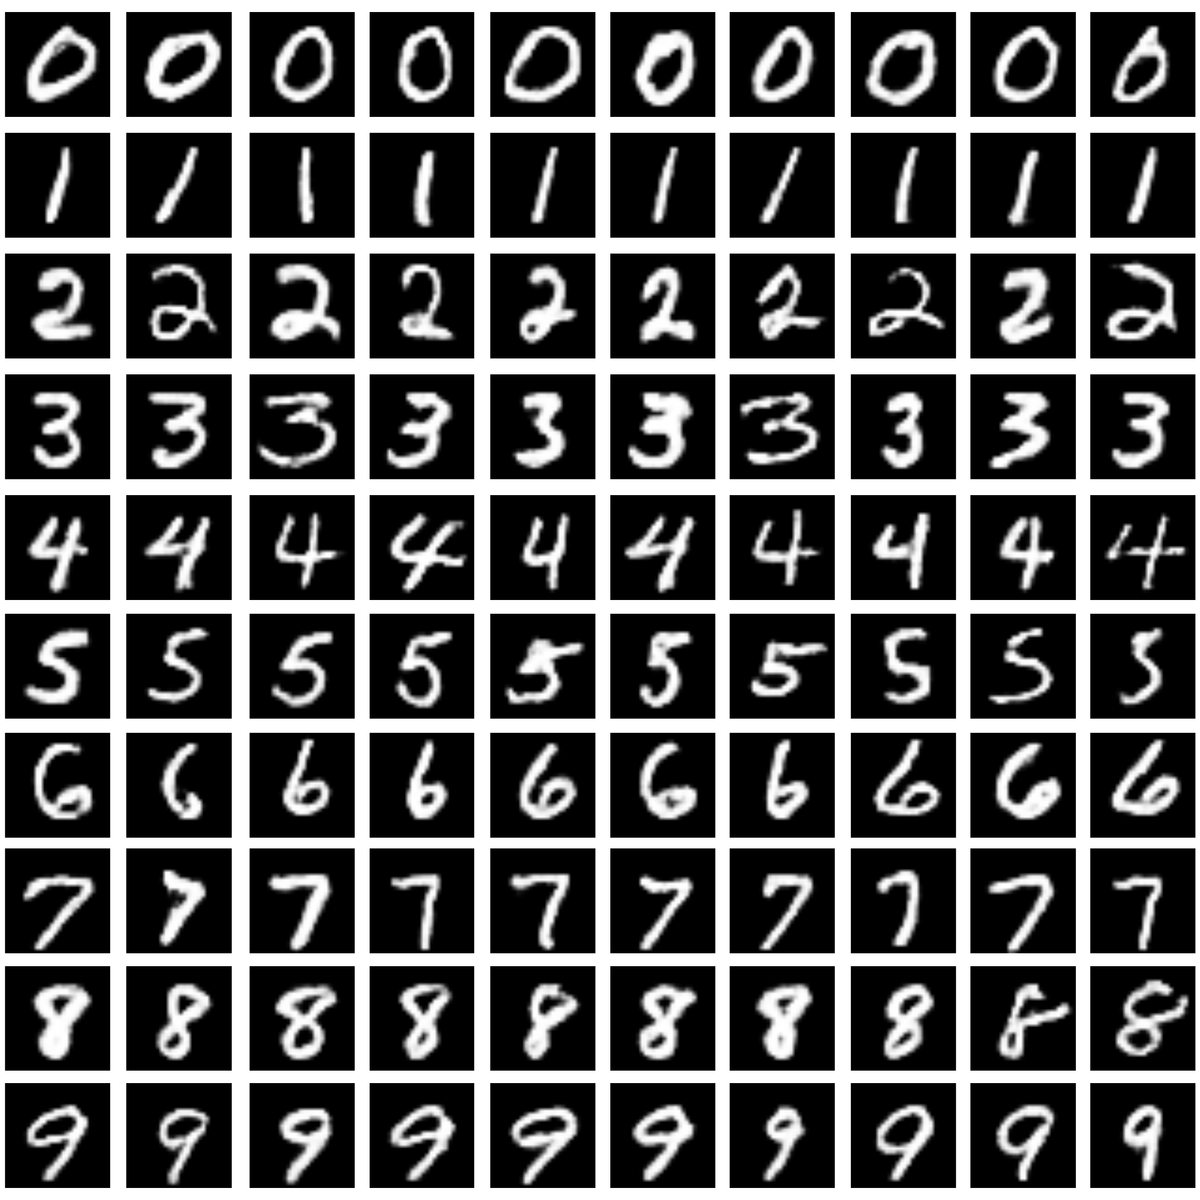
\includegraphics[width=0.5\textwidth]{figures/dataset-card.png}
  \caption{Each digit drawn out clearly}
\end{figure}

\end{frame}
\begin{frame}
  \frametitle{An  Example}
  \begin{enumerate}
\item Each image is a set of \(p\) pixels, or a vector \(\vec{v} = (v_1, v_2, \cdots , v_p)\). Each element \(v_i\) tells us how 'dark' or 'light' that pixel is. 0 is black, and 1 is white.
          \pause
          \item We can say that we have \(M\) vectors \(\vec{v}\) in \(p\) -dimensional space or \(\mathbb{R}^{p}\)
  \end{enumerate}

\end{frame}
\end{document}

\message{ !name(slides.tex) !offset(-60) }
